\section{Data}
\subsection{Current Data Set}
\label{sec:data}

Samples are filtered from the dataset introduced in our previous studies \cite{pooyan_esem}, \cite{pooyan_qrs}, which provides compilability and software quality metrics across 68 open-source Java projects owned by Apache, Google, and Netflix. 
This study is performed on 914 commits, 314 uncompilable and 600 compilable.

\begin{figure}[htbp]
    \centerline{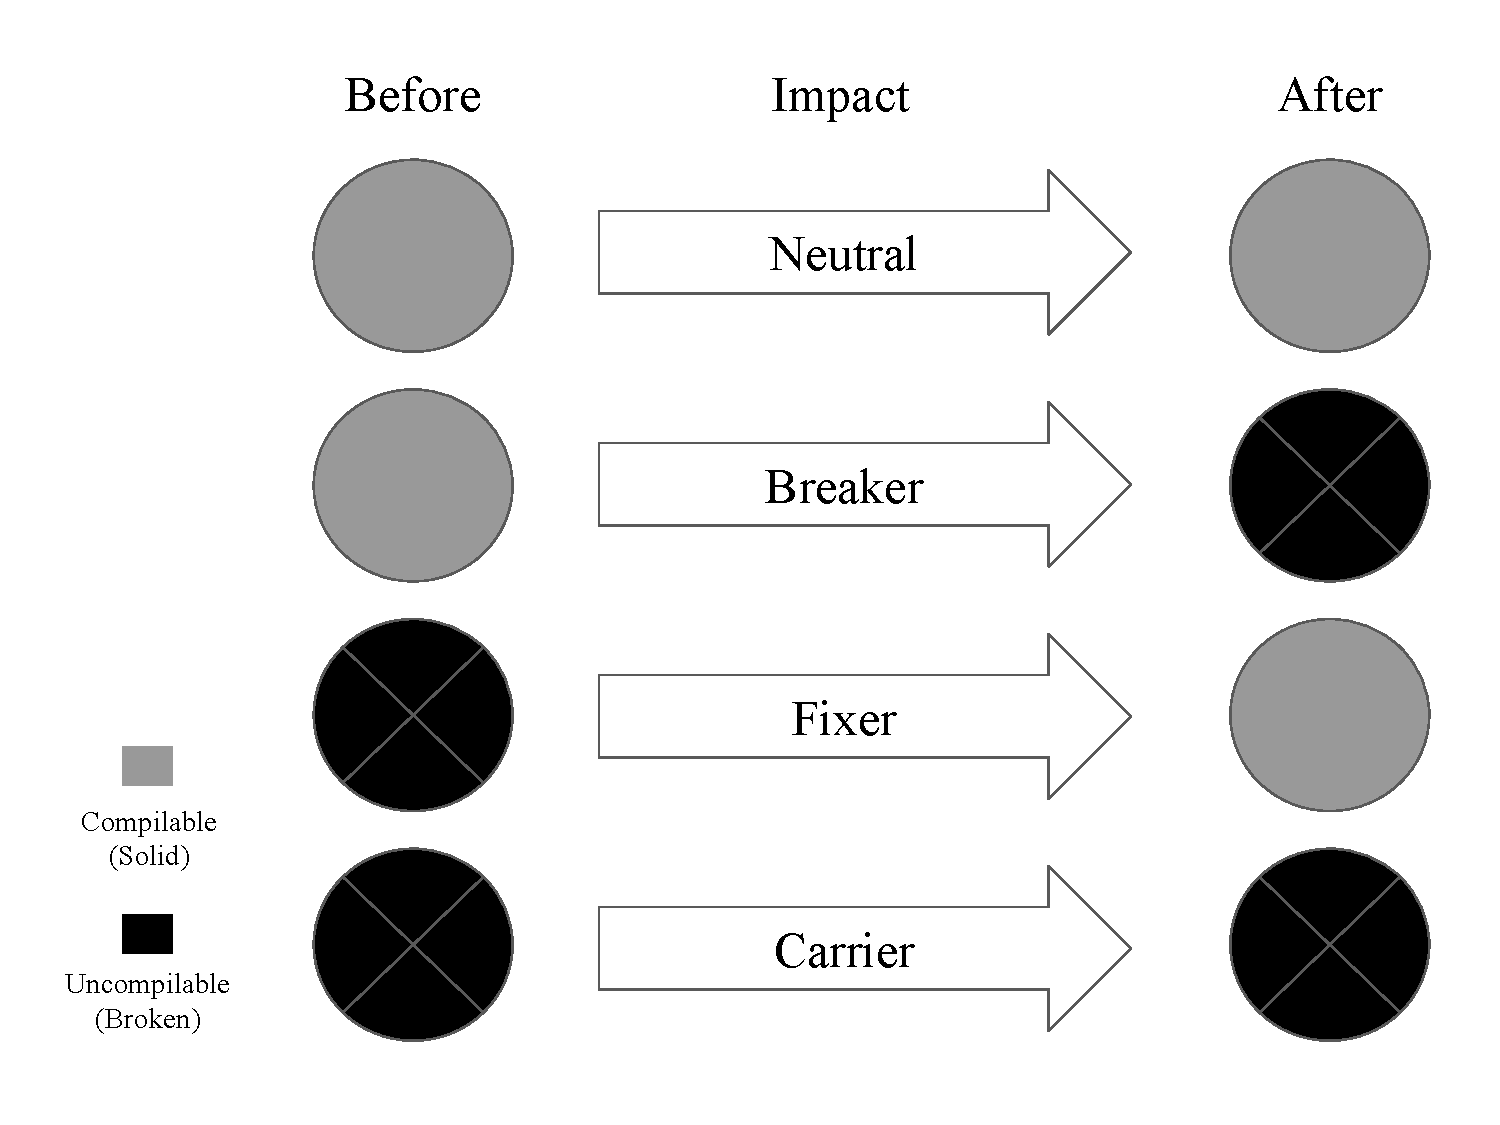
\includegraphics[scale=0.3]{figures/terminology.pdf}}
    \caption{Four Types of Impactful Commit}
    \label{fig:terminology}
    \end{figure}

We use the following terminology, as shown in Fig. \ref{fig:terminology}, to categorize commits based on their impact on compilability. 
A core module is a module that contains the majority of the source code, such as the main modules in most Apache library systems.
A commit is \textit{impactful} if it changes a core module.
An impactful commit is \textit{broken} if it creates an uncompilable revision; otherwise, it is \textit{solid}.
A broken commit is a \textit{breaker} if it breaks the compilability of its solid parent; otherwise, it is a \textit{carrier}.
A solid commit is a \textit{fixer} if it fixes its broken parent; otherwise it is \textit{neutral}.
Fig. \ref{fig:sequence} shows an example of a commit sequence with these four types of impactful commit.

\begin{figure}[htbp]
    \centerline{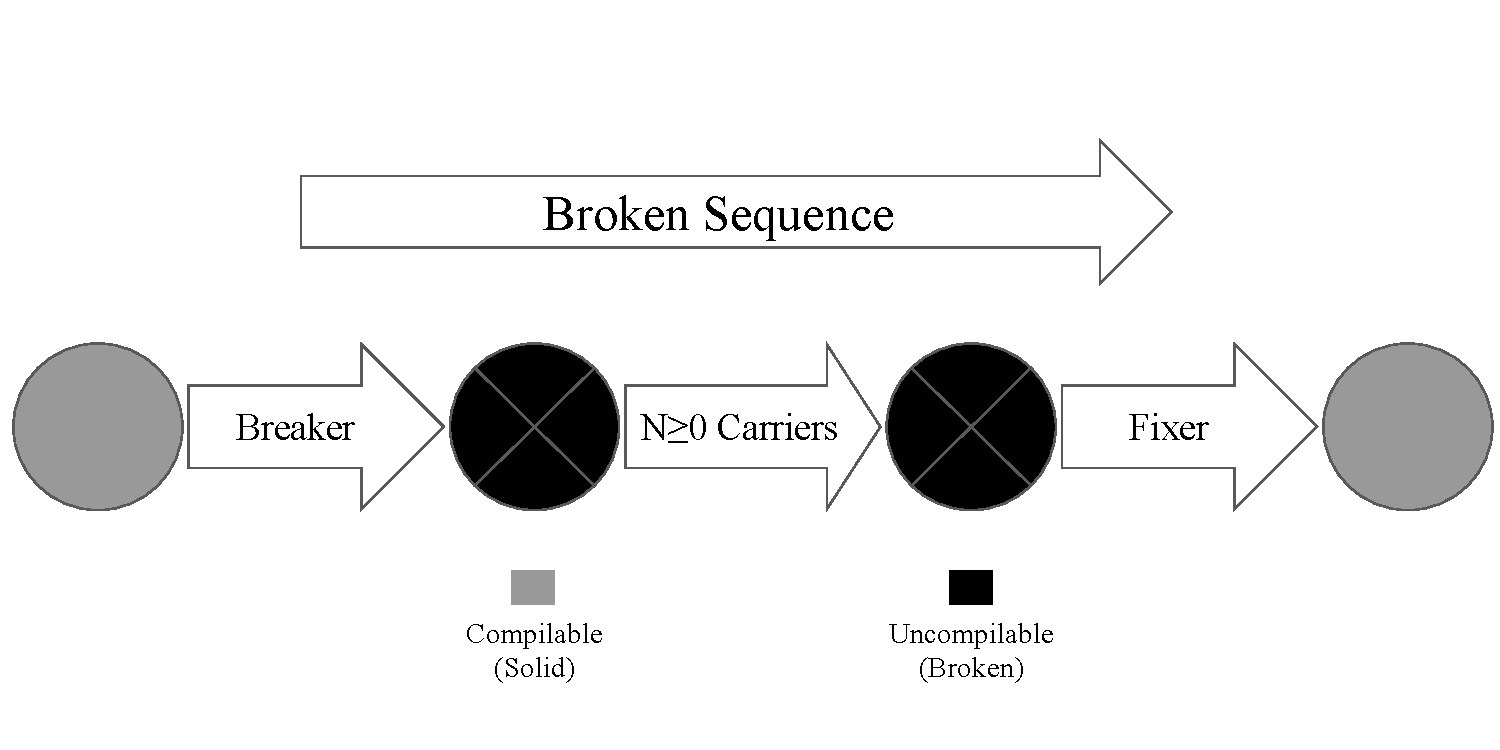
\includegraphics[scale=0.3]{figures/sequence.pdf}}
    \caption{An Example of a Broken Sequence}
    \label{fig:sequence}
    \end{figure}

We do not categorize orphan or merge commits into breaker, carrier, fixer, or neutral as their impact is not identifiable by comparing two software revisions (i.e., before and after).

For selecting subject systems, we retrieve all Java projects owned by Google and Netflix from GitHub.
We select a system only if it 1) requires Ant, Maven, or Gradle for compilation and is not an Android, a Bazel, or an Eclipse project, 2) does not require manual installation of other tools (e.g., Protoc) for compilation, 3) is an official product of the organization, and 4) has a core module containing a substantial amount of code.
We target the core module and identify impactfuls in each system and exclude those with fewer than 100 distinct revisions.
For selecting Apache subject systems, we use the same criteria as Netflix and Google, except that we only consider subject systems with fewer than 3000 commits by April 2017.

To develop the commit purpose taxonomy, we analyze 100 commits, using both the code and commit message in deriving the categorization. We consult with Hindle et al. to clarify category definitions, which help to determine the categories included in our final taxonomy. 
In order to apply this taxonomy to small commits, we create further refinements of the definitions for four kinds of tasks. 

We use the resulting categorization taxonomy to tag our dataset of 914 commits. Each commit is labelled and cross-validated by multiple individuals. 
Initial inconsistencies in tagging arise from ambiguities in the original taxonomy. 
To resolve these ambiguities, we study each inconsistent tag, identify the source of confusion and further refine the taxonomy definitions. 
The tag definitions are now more narrow in scope, and overlapping meaning between category definitions is reduced. 
This methodology ensures that our taxonomy can be applied consistently across varied tagging interpretations. 

We also define a threshold for identifying commit size, and use this to label each commit -- \textit{large} or \textit{small}. 
Some related works have introduced thresholds to differentiate between large and small commits; however, our dataset exhibits a narrower range in commit size. 
The average commit size is also reduced due to our focus on the changes within a commit, as opposed to cumulative commit size. 
Thus, based on our dataset, we create a new threshold which defines commit size as the sum of added and deleted lines of code. The 314 uncompilable commits were split into two parts, with the smallest 157 commits labeled \textit{small}, and the remaining 157 commits labeled \textit{large}. 
The resulting threshold -- 184 lines of code -- is used to label the 600 compilable commits.
This threshold is based on the distribution of uncompilable commits in order to motivate discussions on the relative sizes and categorization of uncompilable commits. The final dataset contains 157 each of large and small uncompilable commits, and 138 \& 462 large and small compilable commits, resp.

To analyze software quality evolution over uncompilable commits in relation to the quality of compilable commits, we examine metrics on code complexity, maintainability, and security, provided by SonarQube \footnote{https://www.sonarqube.org/} and PMD \footnote{https://pmd.github.io/}. As uncompilable commits cannot be directly assessed by dynamic software quality analysis, we measure the overall quality change in the compilable commits before and after uncompilable sequences, extrapolating to determine the individual quality of each commit. 


\subsection{Additional Data to be Collected}
